\documentclass[a4paper,14pt]{extarticle}

\usepackage[left=30mm, right=10mm, top=20mm, bottom=20mm]{geometry}

\usepackage[T2A]{fontenc}
\usepackage[utf8]{inputenc}
\usepackage[russian]{babel}
\usepackage{tempora}
\usepackage{type1cm}
\usepackage{indentfirst}

\usepackage{minted}
\usepackage{xcolor}

\usepackage{siunitx}
\usepackage{booktabs}
\usepackage{multirow}


\usepackage{csquotes}
\usepackage[
    parentracker=true,
    backend=biber,
    style=gost-numeric,
    sorting=nty
]{biblatex}

\usepackage[nodisplayskipstretch]{setspace}
\usepackage[none]{hyphenat}
\usepackage{fancyhdr}
\usepackage{titlesec}
\usepackage{tocloft}

\usepackage{amssymb}
\usepackage{amsmath}
\usepackage{tikz}
\usepackage{pgfplots}
\usepackage{graphicx}
\usepackage{caption}
\usepackage{subcaption}
\usepackage[hidelinks]{hyperref}
\usepackage[russian]{cleveref}
\usepackage{bookmark}

\pgfplotsset{compat=1.18}

\onehalfspacing
\sloppy

\pagestyle{fancy}
\fancyhf{}
\fancyfoot[R]{\thepage}
\renewcommand{\headrulewidth}{0pt}

\definecolor{codebg}{rgb}{0.12,0.12,0.14}
\definecolor{codeframe}{rgb}{0.40,0.40,0.45}
\definecolor{keywordcolor}{rgb}{0.45,0.65,1.0}
\definecolor{stringcolor}{rgb}{1.0,0.55,0.45}
\definecolor{commentcolor}{rgb}{0.55,0.75,0.60}
\definecolor{textcolor}{rgb}{0.90,0.90,0.90}

\renewcommand{\theFancyVerbLine}{
	\sffamily\small\color{black}\arabic{FancyVerbLine}
}

\setminted{
    bgcolor=codebg,
	fillcolor=codebg,
	framesep=1em,
	frame=single,
    rulecolor=\color{codeframe},
    fontsize=\normalsize,
    baselinestretch=1.1,
    linenos,
    numbersep=6pt,
    tabsize=4,
    breaklines,
    breakbytoken,
	breaksymbolleft={},
    autogobble,
    showspaces=false,
    showtabs=false,
}

\usemintedstyle{lightbulb}
\setmintedinline{
    bgcolor=codebg
}

\makeatletter
\setlength{\@fptop}{0pt}
\setlength{\@fpsep}{8pt}
\setlength{\@fpbot}{0pt plus 1fil}
\makeatother

\newcommand{\circledequals}{\mathbin{\tikz \node[draw,circle,inner sep=1pt] {$=$};}}

\begin{document}
    \begin{titlepage}
		\centering
		
		
\includegraphics{images/FEFU-logo.jpg}\\
		МИНИСТЕРСТВО ОБРАЗОВАНИЯ И НАУКИ РОССИЙСКОЙ ФЕДЕРАЦИИ\\
		Федеральное государственное автономное образовательное учреждение высшего образования\\
		\textbf{«Дальневосточный федеральный университет»}

		\rule{\linewidth}{0.8mm}\\[0.3cm]
		
		\textbf{ИНСТИТУТ МАТЕМАТИКИ И КОМПЬЮТЕРНЫХ ТЕХНОЛОГИЙ}\\
		\textbf{Кафедра математического и компьютерного моделирования}\\
		\vspace*{0.9cm}
		
		Кулахсзян Сергей Грайрович\\
        \vspace*{0.3cm}

		ЛАБОРАТОРНАЯ РАБОТА № 3 \\
        ЗАДАЧА № 18 \\
		\vspace*{0.5cm}

		\textbf{Задачи на реактивное движение}\\
		\vspace*{0.5cm}

		Направление подготовки 02.03.01сцт Сквозные цифровые технологии,\\ 
        бакалавриатская программа «Математика и компьютерные науки»\\ 
        Очной формы обучения\\
		\vspace{1.5cm}

		
		\vfill
		\centering
		г. Владивосток\\
		2026
	\end{titlepage}

    \tableofcontents
    \thispagestyle{empty}

	\newpage
    \pagenumbering{arabic}
    \setcounter{page}{3}
    \section{Постановка задачи}
    Ракета с нулевой начальной скоростью движется под действием отдачи от струи газа, исходящей со скоростью 2 км/с.
    Масса ракеты с полным запасом топлива равна 400 т, без топлива -- 50 т.
    Пренебрегаются силы тяжести и сопротивления воздуха.
    
    Какова будет скорость ракеты после сгорания всего топлива?

    \section{Математическое моделирование}
    По закону Мещерского движение тела с переменной массой можно записать формулой:
    \begin{equation} \label{Mesherskiy_formula}
        m(t) v'(t) = F(t) + u(t) m'(t),
    \end{equation}
    где $m(t)$ -- масса ракеты в момент времени $t$ (в секундах), $v(t)$ -- скорость (в км/с) ракеты в момент времени $t$, $F(t)$ -- действующая на ракету сила в момент времени $t$, $u(t)$ -- относительная скорость частиц (в нашем случае это скорость газовой струи).
    
    Так как силы пренебрегаются, то $F(t) = 0$.
    Также по условию нам дана скорость струи газа, она у нас постоянна и равна -2, так как газовая струя идет в противоположном направлении.
    
    Подставляя эти условия в (\ref{Mesherskiy_formula}), получаем:
    \begin{equation} \label{our_Mesherskiy_formula}
        m(t) v'(t) = -2 m'(t).
    \end{equation}

    В конечный момент времени $T$ топливо будет полностью израсходовано, то есть $m(T) = 50$.
    

    Совершим некоторые преобразования в формуле (\ref{our_Mesherskiy_formula}), чтобы прийти к зависимости скорости от массы: \\
    $\displaystyle
    m(t) \frac{dv}{dt} = -2 \frac{dm}{dt} \\
    m dv = -2 dm \\
    dv = -2 \frac{dm}{m}. \\
    $
    Тогда математическая модель будет иметь вид:
    \begin{equation*}
        \begin{cases}
            \displaystyle v'(m) = -\frac{2}{m} \\
            v(m_0) = v_0
        \end{cases}.
    \end{equation*}

    Так как в начальный момент времени скорость нулевая, следует, что топливо пока не было истрачено, то есть $m_0 = 400$ при $v_0 = 0$.
    \begin{equation} \label{model}
        \begin{cases}
            \displaystyle v'(m) = -\frac{2}{m} \\
            v(400) = 0
        \end{cases}.
    \end{equation}

    \section{Аналитическое решение}
    Уравнение (\ref{model}) имеет следующее решение: \\
    $\displaystyle
    dv = -2 \frac{dm}{m} \\
    v(m) = -2 \ln m + c \\
    v(400) = -2 \ln 400 + c = 0 \Rightarrow c = -2 \ln 400 \\
    v(m) = 2 \ln \frac{400}{m} \\
    v(50) = 2 \ln 8 \approx 4.16 \text{ км/с}. \\
    $
    Тогда получаем, что скорость ракеты после сгорания всего топлива примерно равно 4.16 км/с.

    \section{Численное решение}
    Для численного решения уравнений был применён метод Рунге-Кутта 4-го порядка, но в обратном направлении: \\
    $\displaystyle
    v_{i - 1} = v_i - \frac{h}{6} (k_1 + 2k_2 + 2k_3 + k_4) \\
    k_1 = f(m_i, v_i) \\
    k_2 = f \left( m_i - \frac{h}{2}, v_i - \frac{h}{2} k_1 \right) \\
    k_3 = f \left( m_i - \frac{h}{2}, v_i - \frac{h}{2} k_2 \right) \\
    k_4 = f(m_i - h, v_i - h k_3)
    $

    Вычисление было произведено на отрезке $[50; 400]$ при значениях $N = 10; 100; 1000$.
    В ходе выполнения были получены следующие результаты, представленные на графиках:

    \begin{figure}[H]
        \centering
        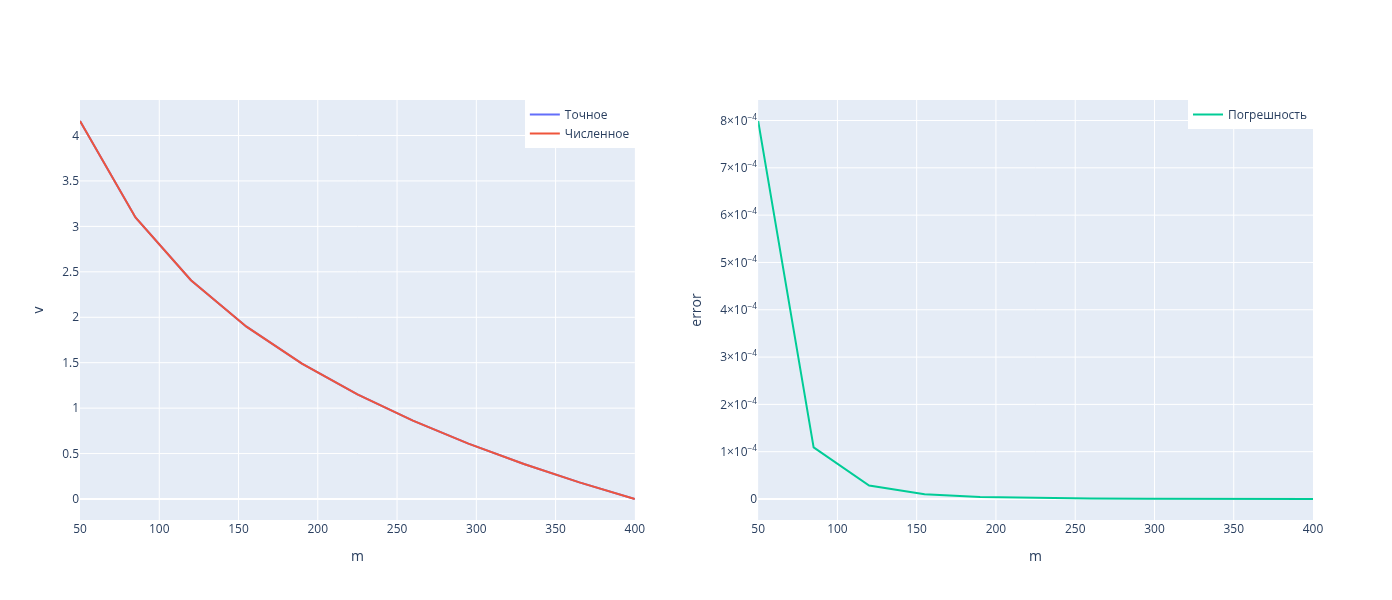
\includegraphics[width=\textwidth]{images/10.png}
        \caption{Тестирование решения при $N = 10$}
        \label{n_10}
    \end{figure}

    \begin{figure}[H]
        \centering
        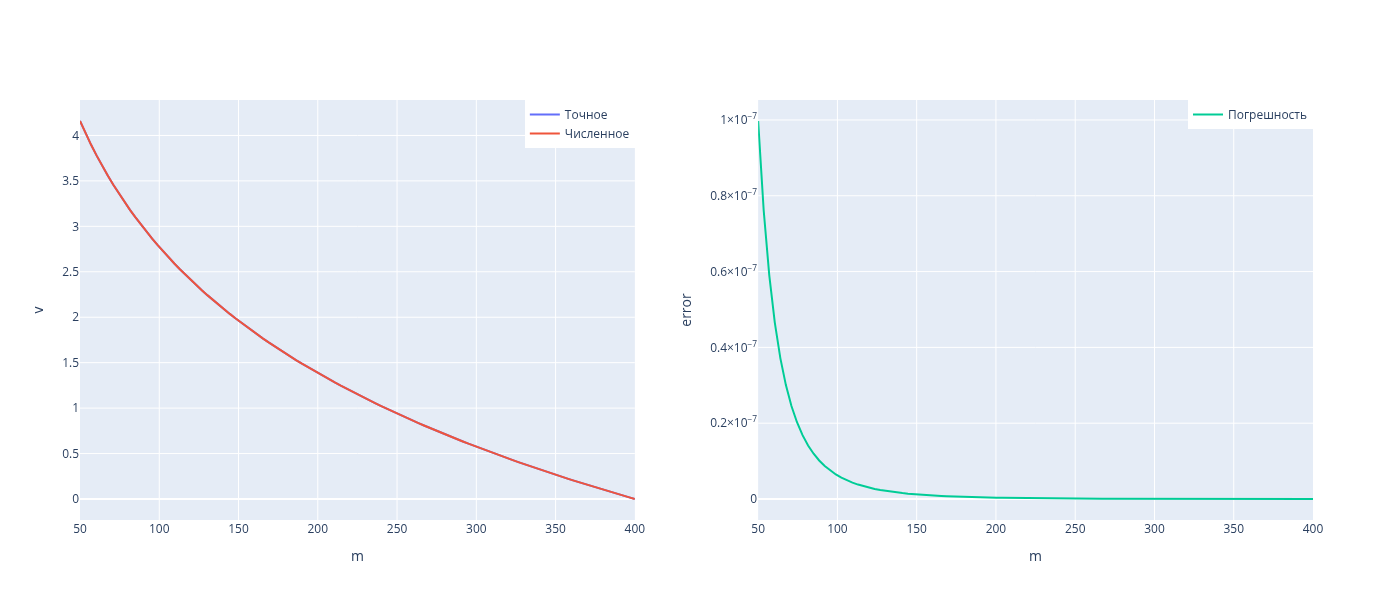
\includegraphics[width=\textwidth]{images/100.png}
        \caption{Тестирование решения при $N = 100$}
        \label{n_100}
    \end{figure}

    \begin{figure}[H]
        \centering
        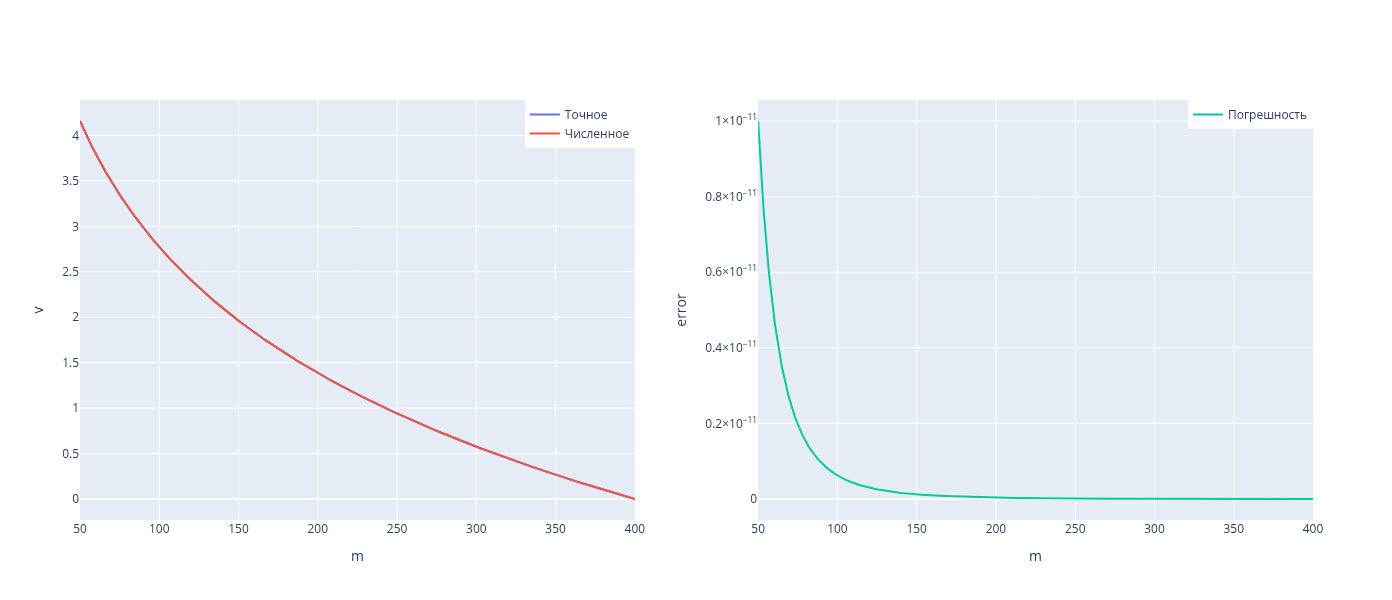
\includegraphics[width=\textwidth]{images/1000.png}
        \caption{Тестирование решения при $N = 1000$}
        \label{n_1000}
    \end{figure}

    \section{Заключение}
    В ходе лабораторной работы была рассмотрена и решена задача на реактивное движение. 
    Сравнение численных и аналитических решений, приведённое на графиках (\cref{n_10}, \cref{n_100}, \cref{n_1000}), показало, что при увеличении числа узлов сетки численное решение всё точнее приближается к аналитическому.
    Ответ был получен 4.16 км/с.
\end{document}